
\chapter{Modeling} \label{ch:modeling}

Writing a modeling chapter in an engineering thesis involves a structured and comprehensive approach to presenting the conceptualization, design, and analysis of the model. This chapter serves as a bridge between theoretical understanding and practical application, showcasing the technical prowess of the researcher. Begin by clearly defining the purpose and scope of the model, outlining the problem it addresses, and highlighting its significance in the context of the broader field. Detail the assumptions and simplifications made during model development, discussing the underlying mathematical equations, physical principles, or algorithms employed. Offer clarity on the model's inputs, parameters, and variables, providing justifications for their selection. Present the model's design process step-by-step, including numerical methods or software tools used for simulations. Visual aids, such as graphs, diagrams, and schematics, can enhance clarity and comprehension. Discuss validation efforts by comparing model predictions with experimental or empirical data. Address the limitations and uncertainties associated with the model, highlighting areas for future refinement. Concluding with a summary of key findings and their implications solidifies the chapter's role in contributing to the understanding of complex engineering phenomena. \medskip

Here illustrations can be helpful as the one shown in~\figref{fig:sys-schematic}.

%
\begin{figure}[h]
	\begin{small}
		\begin{center}
			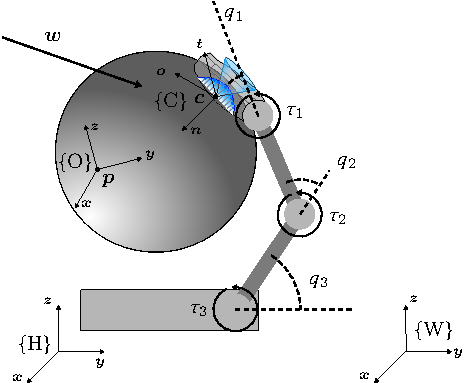
\includegraphics[width=0.6\textwidth]{chapters/modeling/fig/sys-schematic-reversed-crop.pdf}
		\end{center}
		\caption{example system illustration.}
		\label{fig:sys-schematic}
	\end{small}
\end{figure}
